\usetikzlibrary{patterns}
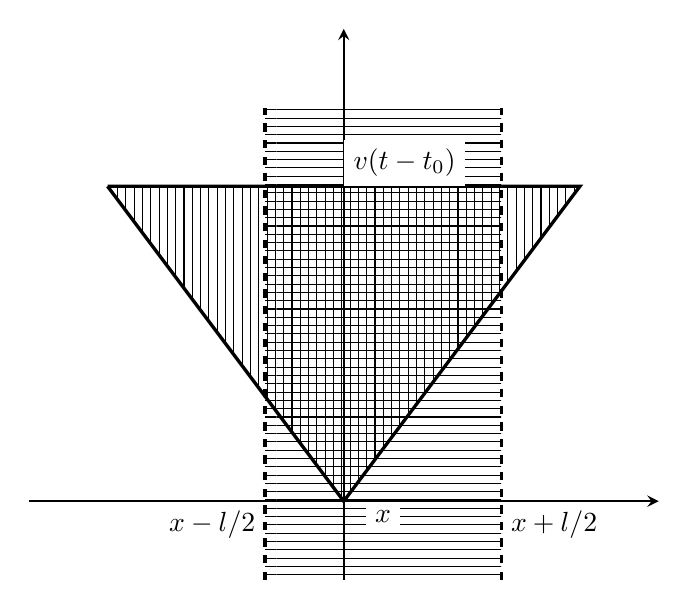
\begin{tikzpicture}

\draw[thick,-stealth]  (0,-1) -- (0,6);
\draw[thick,-stealth] (-4,0) -- (4,0);
\draw[very thick, pattern=vertical lines] (-3,4) -- (3, 4) -- (0,0) -- (-3, 4);
\draw[very thick, dashed] (2, -1) -- (2, 5);
\draw[very thick, dashed] (-1, -1) -- (-1, 5);
\path[pattern=horizontal lines] (2, -1) rectangle (-1, 5);

\node[below, fill = white] at (0.5,0) {$x$};
\node[above right, fill = white] at (0,4) {$v(t - t_0)$};
\node[below left] at (-1,0) {$x - l/2$};
\node[below right] at (2,0) {$x + l/2$};

\end{tikzpicture}